\documentclass[aspectratio=1610]{beamer}

\usepackage{amsmath}
\usepackage{multirow}
\usepackage{url}
\usepackage{hyperref}

\hypersetup{
colorlinks=false,
}

\usepackage{listings,calc,graphicx}

\title % [short title] (optional, use only with long paper titles)
{CPSC 1000: Introduction to Computer Science}

\subtitle{Reading the voltage of an analog signal} % (optional)

\author{Robert Benkoczi, C556\\\url{robert.benkoczi@uleth.ca}}
\date{25-Sep-2018\\(Week 3)}

% for figures created with IPE
%\pdfpagebox5

\lstloadlanguages{C}
\lstset{language=C,tabsize=2,aboveskip=-22pt,belowskip=-22pt,keepspaces,
  basicstyle=\small\ttfamily,}


\begin{document}

\begin{frame}[plain]
\titlepage
\end{frame}

%%%%%%

\begin{frame}[t,plain]{Objectives}
\begin{itemize}
\item Using the Lab Manual and the sample code available on Moodle,
  students will correctly connect a device generating an analog signal
  to the Arduino.
\item Students will write code to measure the analog signal.
\item Students will output information from the Arduino board to the
  serial monitor window on the workstation.
\end{itemize}
\end{frame}


%%%%%%

\begin{frame}[t,plain]{Motivation}
\begin{itemize}
\item Many inexpensive sensors transmit their information through an
  analog signal. The code we use in this activity can also be used to
  read these sensors (ex: light, sound, temperature, etc.)
\item A potentiometer can also be used as a form of input for an
  Arduino project (ex: to configure the device).
\end{itemize}
\end{frame}




%%%%%%

\begin{frame}[t,plain]{Reading an analog signal}
\framesubtitle{Analog to digital conversion (ADC)}

\end{frame}


%%%%%%

\begin{frame}[t,plain]{Applications}
\framesubtitle{Recording sound}

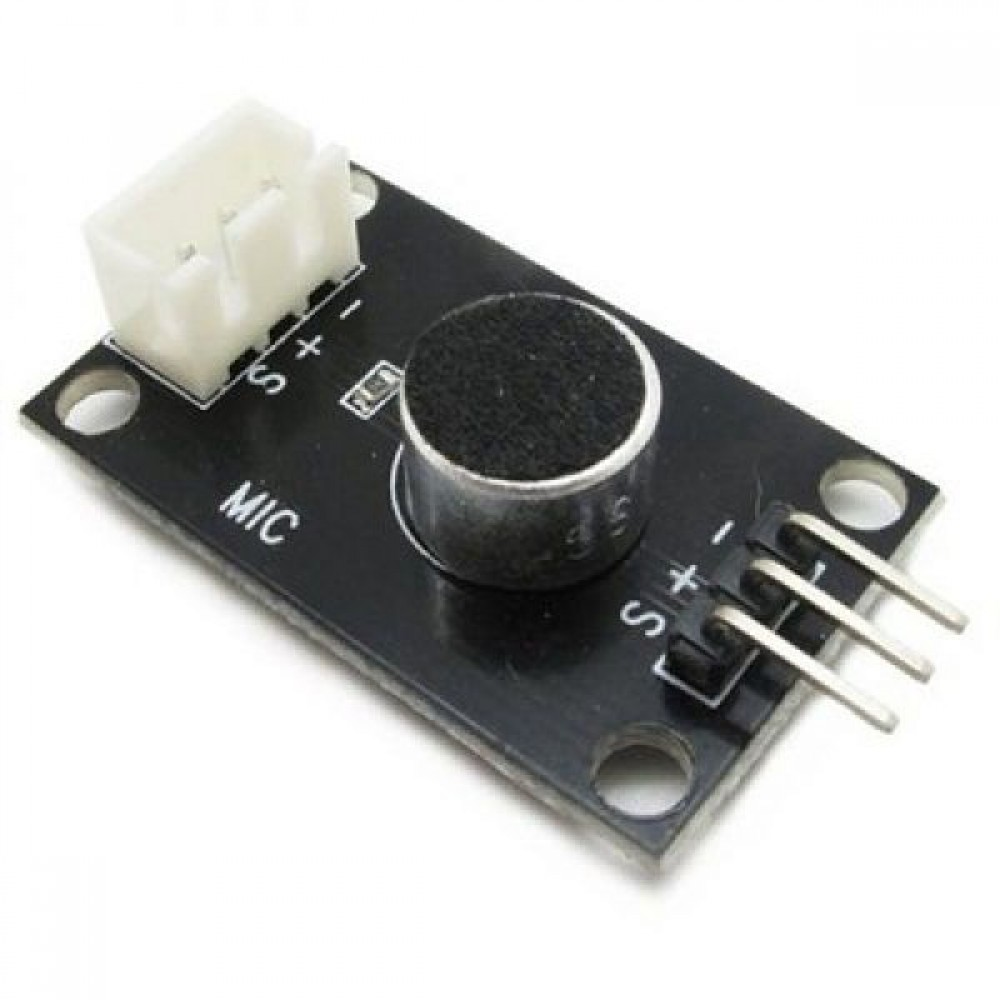
\includegraphics[width=.3\textwidth]{figs/3-sound-sensor.jpg}
\end{frame}


%%%%%%

\begin{frame}[t,plain,fragile]{Code to read an analog signal}

\bigskip
\begin{semiverbatim}
\begin{lstlisting}
int val = analogRead(pin_number);
\end{lstlisting}
\end{semiverbatim}

\end{frame}


%%%%%%

\begin{frame}[t,plain]{Simulating an analog signal with potentiometer}
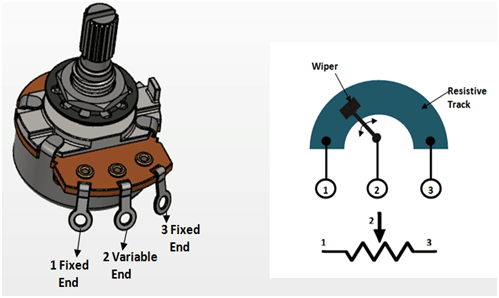
\includegraphics[width=.3\textwidth]{figs/3-potentiometer-pinout.png}
\end{frame}


%%%%%%

\begin{frame}[t,plain,fragile]{Serial communication}
\framesubtitle{Sending data to the workstation - println}

\bigskip
\begin{semiverbatim}
\begin{lstlisting}
Serial.begin(speed);
\end{lstlisting}
\end{semiverbatim}

\vfill

\begin{semiverbatim}
\begin{lstlisting}
Serial.print(value);
\end{lstlisting}
\end{semiverbatim}

\vfill

\begin{semiverbatim}
\begin{lstlisting}
Serial.println(value);
\end{lstlisting}
\end{semiverbatim}
\end{frame}


%%%%%%

\begin{frame}[t,plain,fragile]{Application}

\smallskip
Sending message: ``Potentiometer value: 99''.
\end{frame}

\end{document}
